
\begin{frame}{Introduction}
    \begin{center}
        \emph{Sidon sets and statistics of the ElGamal function} \\
        \citet*{boppre2020sidon}
    \end{center}
    
    \begin{itemize}
        \item Started in 2016 as a research challenge by Joachim von zur Gathen;
        \item Boppré and Perin wrote a report with experimental analysis;
        \item By 2017, Ana and Joachim wrote the Sidon sets part and submitted to arxiv.
        \item In 2020, the paper was published in Cryptologia.
    \end{itemize}
\end{frame}


\begin{frame}{ElGamal Permutations}

    Let $ G = \Z_p^* = \{1, \ldots, p-1\}$ be a cyclic group of order $d =p-1$,
    
    $p$ prime, and $\Z_d = \{0, \ldots, d-1\}$
    \vspace{10pt}
    
    \pause
    \begin{itemize}
        \item ElGamal signatures use $G = \{ g^x : x\in \Z_d\}$, where $g$ is a generator of $G$;
        \item $g^x$ is a unique representation of $x$, and thus it spans a permutation of $G$.
        \item We want to investigate the randomness of the map $x \to g^x$
    \end{itemize}
    
\end{frame}


\begin{frame}{ElGamal Permutations}

Since want to investigate permutations of $G$, we introduce the following notation.
\vspace{10pt}

\begin{minipage}{.5\textwidth}
	\begin{table}[]
	    \centering
	    \begin{tabular}{c|c}
	        $x$ & $x^\star$ \\ \hline \hline
	        $1$ & $1$ \\
	        $2$ & $2$ \\
	        $\cdots$ & $\cdots$ \\
	        $p-2$ & $p-2$ \\
	        $p-1$ & $0$ 
	    \end{tabular}
	     \caption{$\star: \mathbb{Z}_p^* \rightarrow \mathbb{Z}_d$}
	    \label{tab:xmap}
	\end{table}
\end{minipage}%
\begin{minipage}{0.5\textwidth}
    Now for $x\in G$, we can evaluate the map from $G$ to $G$
    $$x \to g^{x^\star}$$ 
     with respect to its cyclic properties.
\end{minipage}

    
\end{frame}



\begin{frame}{ElGamal Permutations}
Example: Let $p =5$, then $2$ and $3$ are generators of G = $\Z_p^*$.

    \begin{columns}
        \begin{column}{0.45\textwidth}
        \centering
            \begin{table}[]
    	    \begin{tabular}{c|c}
    	        $x$ & $g^{x^\star} $ \\ \hline \hline
    	        $1$ & $2^{1^\star} = 2$ \\
    	        $2$ & $2^{2^\star} = 4$ \\
    	        $3$ & $2^{3^\star} = 3$ \\
    	        $4$ & $2^{4^\star} = 1$  
    	    \end{tabular}
    	    \caption{cycles = \{\{1,2,4\},\{3\}\}}
    	    \label{tab:xmap1}
    	    \end{table}
        \end{column}
        \begin{column}{0.45\textwidth}
    	    \centering
            \begin{table}[]
    	    \begin{tabular}{c|c}
    	        $x$ & $g^{x^\star} $ \\ \hline \hline
    	        $1$ & $3^{1^\star} = 3$ \\
    	        $2$ & $3^{2^\star} = 4$ \\
    	        $3$ & $3^{3^\star} = 2$ \\
    	        $4$ & $3^{4^\star} = 1$
    	    \end{tabular}
    	    \caption{cycles = \{1,2,3,4\}}
    	    \label{tab:xmap2}
    	    \end{table}
        \end{column}
  \end{columns}
  
  \pause
  \begin{itemize}
      \item Distinct $g$ produce distinct permutations;
      \item Distinct $g$ affect the cyclic structures.
  \end{itemize}
  
  We will consider the $\star$ implicit from now on and simply use $g^x$ or $g^x \rem p$.
  
\end{frame}


\begin{frame}{Pictorial Representation}
    \begin{figure}
        \centering
        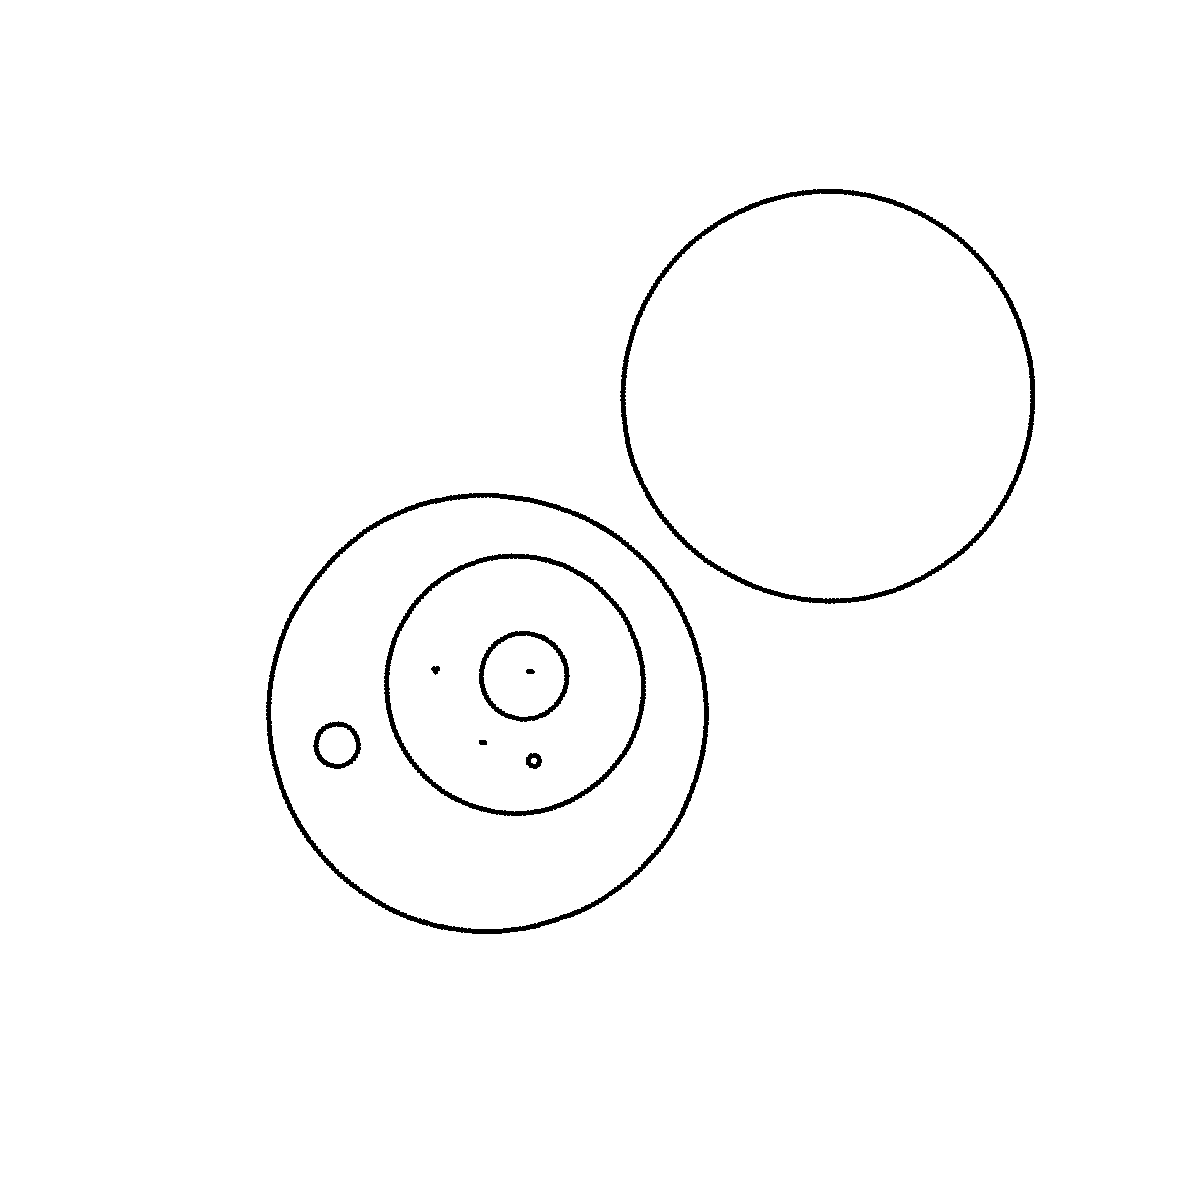
\includegraphics[width=0.7\textwidth]{figures/graph_0011_1009.pdf}
        \caption{$p = 1009$ and $g = 17$}
        \label{fig:smiley}
    \end{figure}
\end{frame}

\begin{frame}{Pictorial Representation}
\begin{tabular}{cc}
        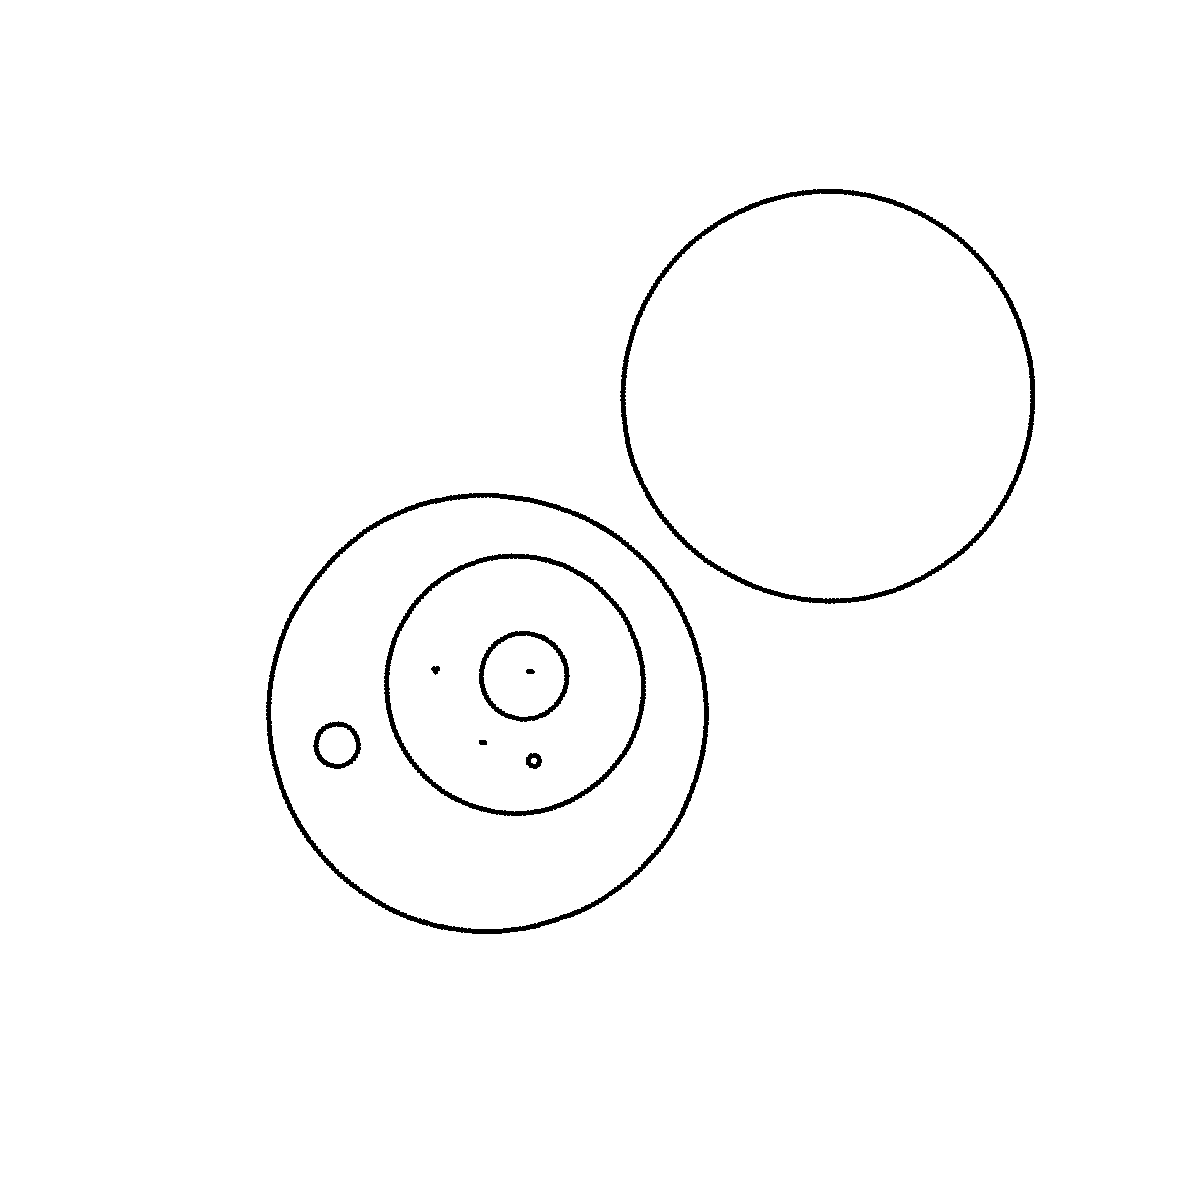
\includegraphics[width=0.4\textwidth]{figures/graph_0011_1009.pdf}
     &  
        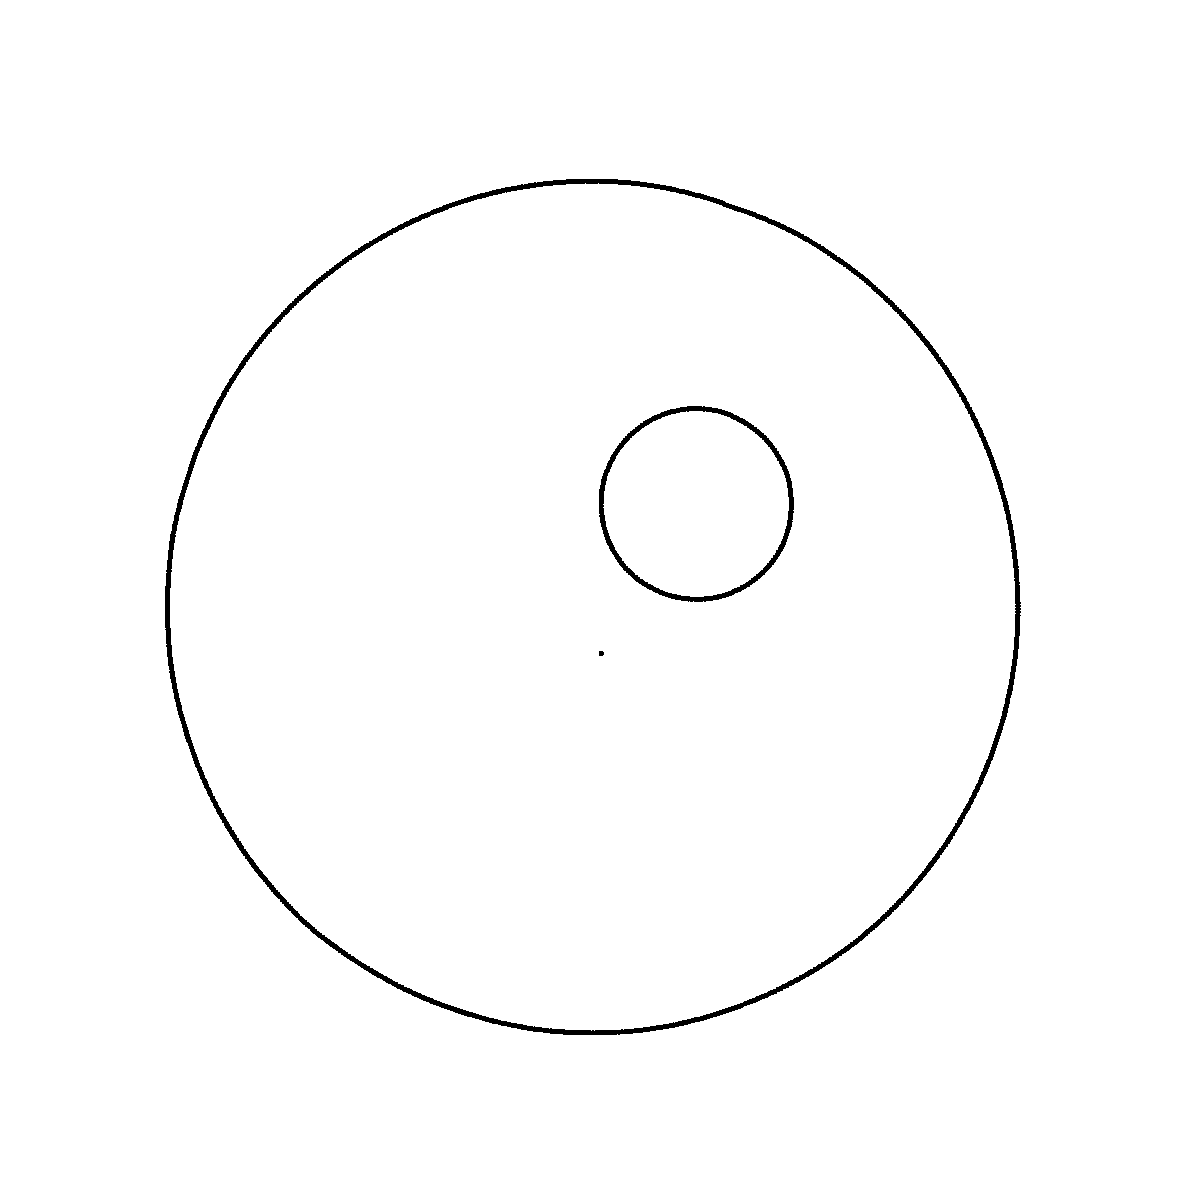
\includegraphics[width=0.4\textwidth]{figures/graph_0017_1009.pdf}
     \\
        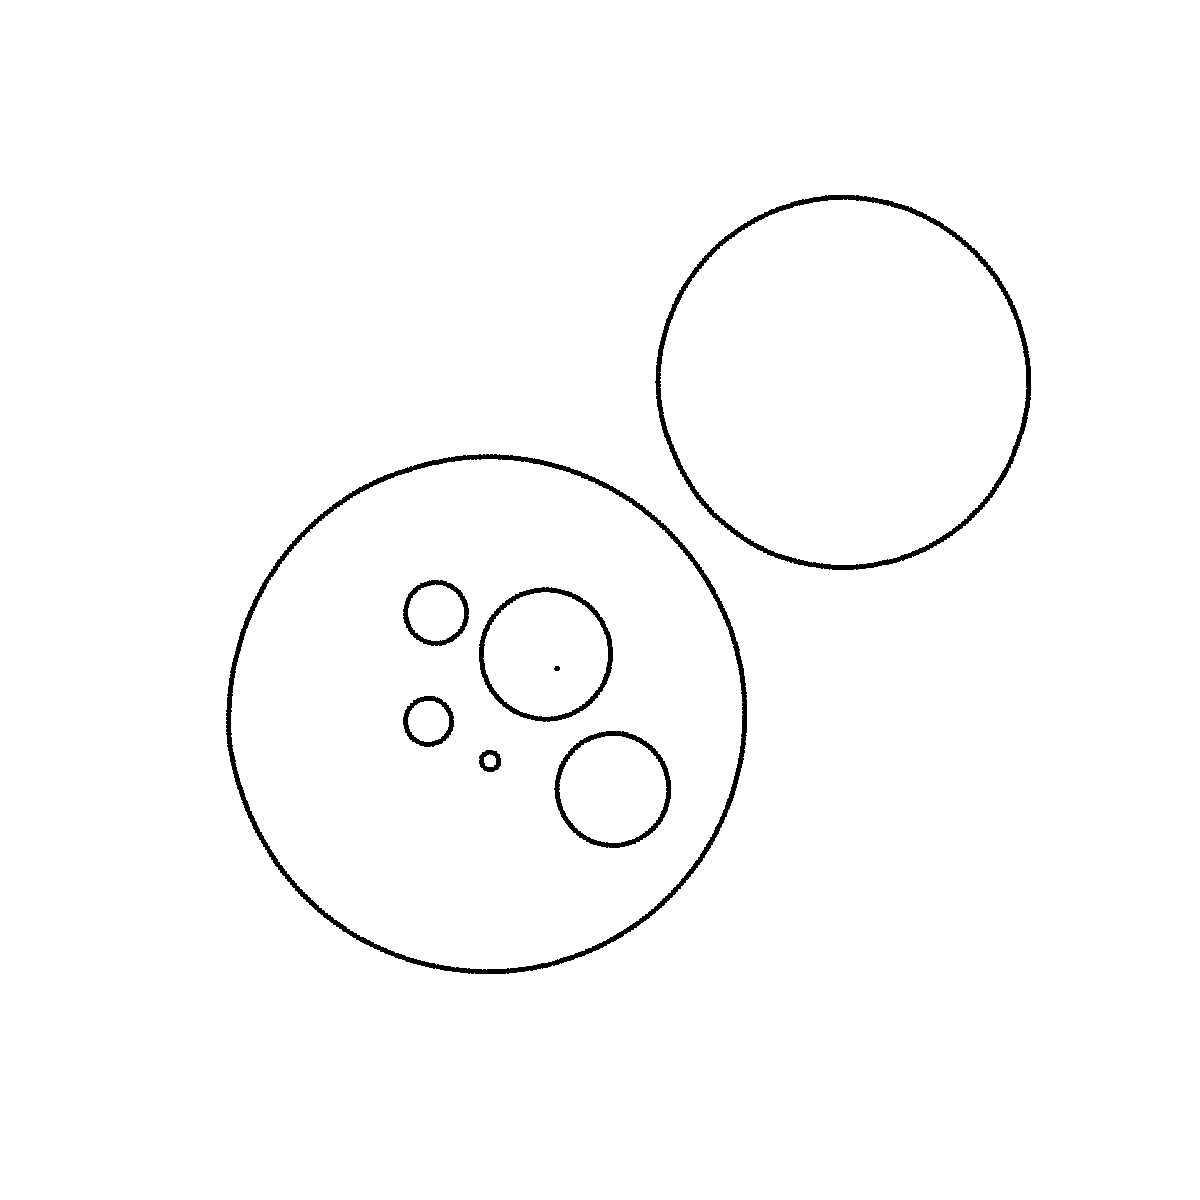
\includegraphics[width=0.4\textwidth]{figures/graph_0022_1009.pdf}
     &  
        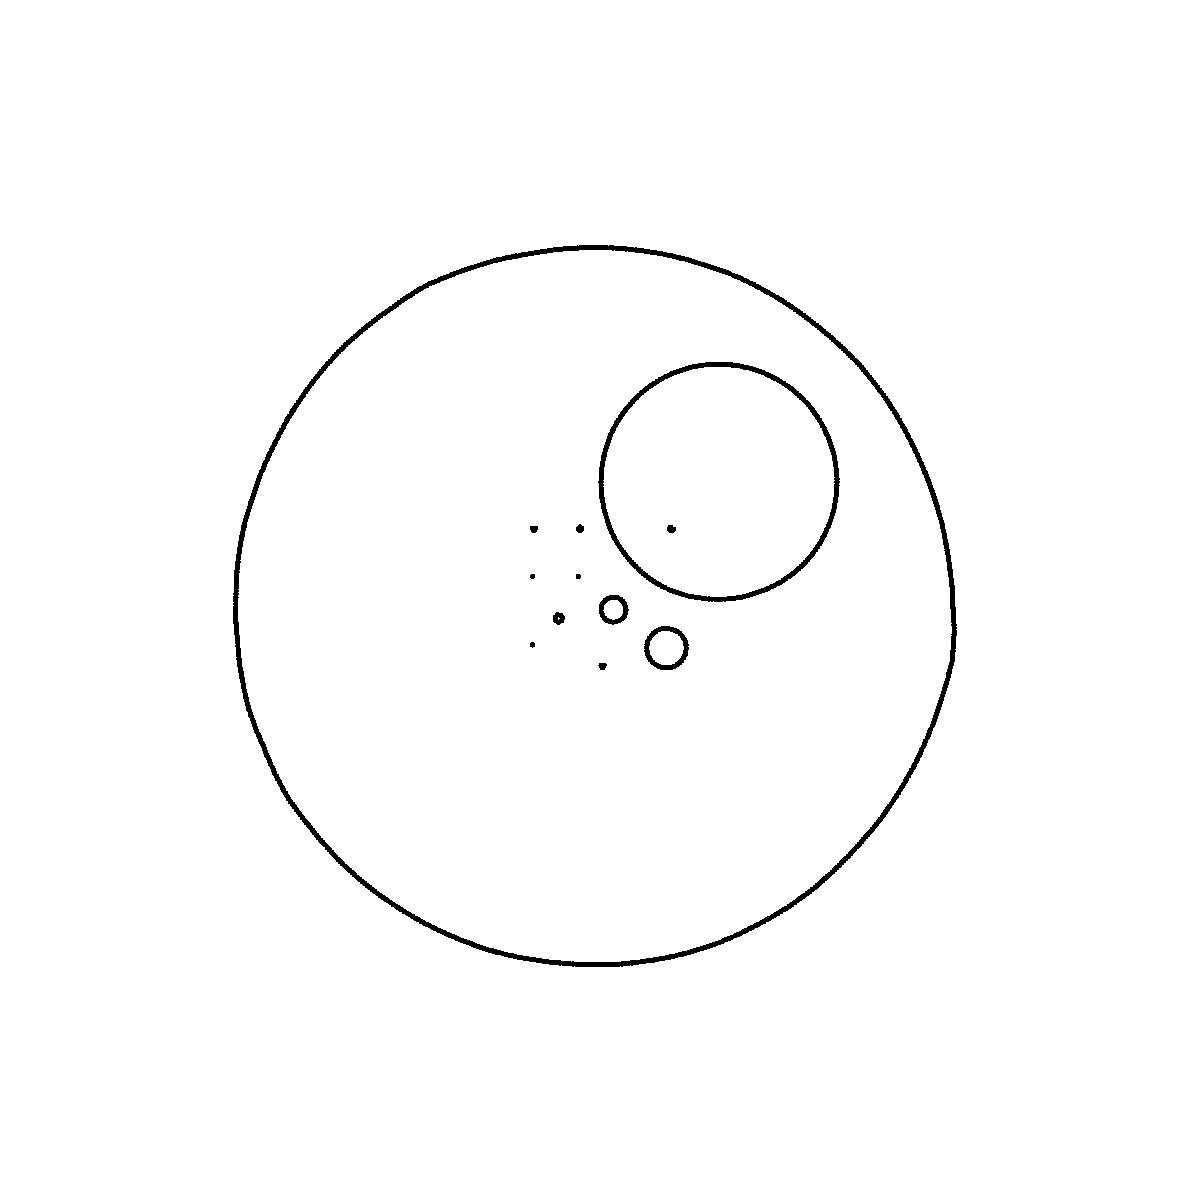
\includegraphics[width=0.4\textwidth]{figures/graph_0026_1009.pdf}
\end{tabular}
\end{frame}

\begin{frame}{Number of cycles}
    \begin{figure}
        \centering
        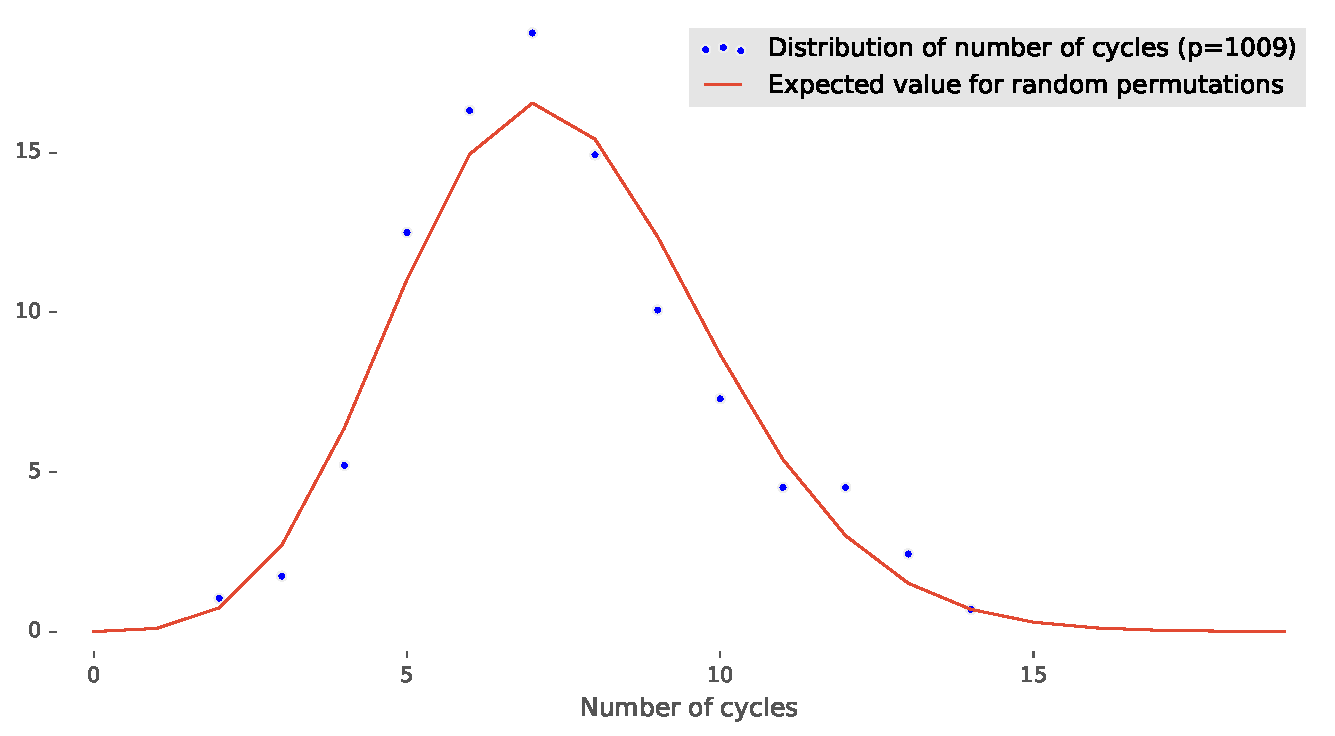
\includegraphics[width=\textwidth]{figures/distribution_of_number_of_cycles_p_1009}
        \caption{Distribution of number of cycles for all 288 generators of $\mathbb{F}_{1009}$}
        \label{fig:elgamalPermCycles}
    \end{figure}
\end{frame}

\begin{frame}{Number of $k$-cycles}
    \begin{figure}
        \centering
        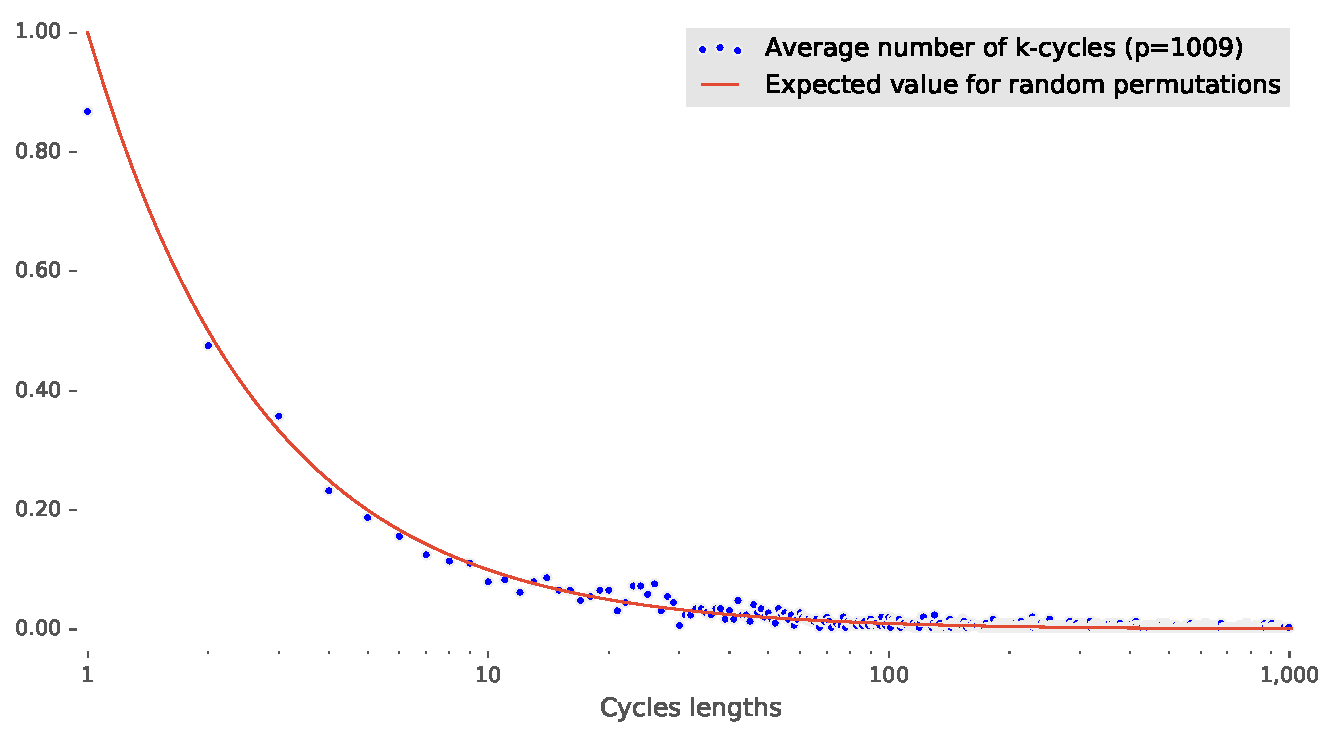
\includegraphics[width=\textwidth]{figures/average_number_of_k_cycles_p_1009}
        \caption{Average number of $k$-cycles in $\mathbb{F}_{1009}$}
        \label{fig:kcycles}
    \end{figure}
\end{frame}

\begin{frame}{Number of fixed points ($k=1$)}
    \begin{figure}
        \centering
        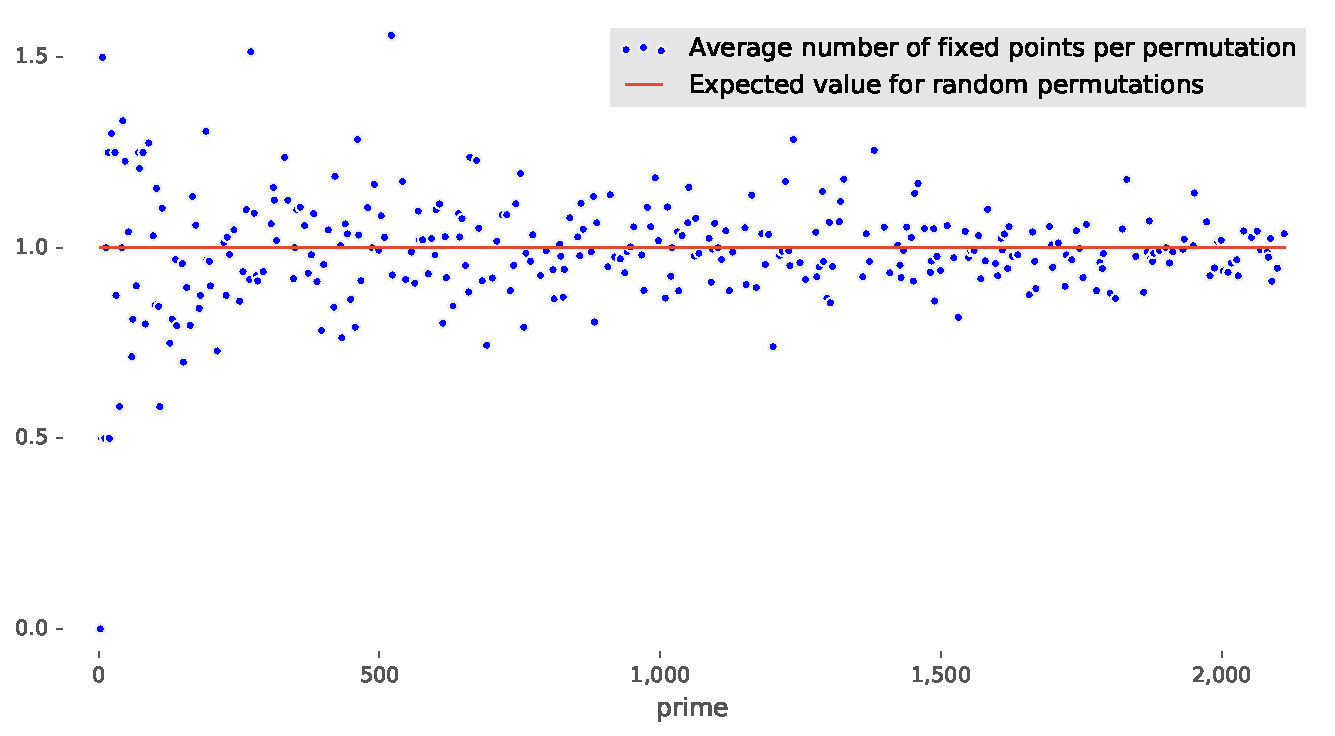
\includegraphics[width=\textwidth]{figures/average_number_of_fixed_points_per_permutation}
        \caption{Average number of fixed points in the generators of $\mathbb{F}_p$}
        \label{fig:fixedpoints}
    \end{figure}
\end{frame}


\begin{frame}{Results with Sidon Sets}
\end{frame}



\begin{frame}{Sequences from permutations}
    For some random permutation $\pi$ in $\mathbb{Z}_p^*$, a $v$-ary sequence $\pi_v\in\mathbb{Z}_v$ is obtained by reducing the permutation modulo $v$:
    \[
        \pi_v = (\pi_0 \rem v, \ldots, \pi_{p-2}\rem v).
    \]
    
    \pause
    \begin{align*}
        \pi &= ( 1, 3, 4, 2) \in \mathbb{Z}_5^*\\
        \pi_2 &= (1, 1, 0, 0) \in \mathbb{Z}_2
    \end{align*}
\end{frame}


\begin{frame}{ElGamal sequences from ElGamal permutations}
    We can do the same for ElGamal Permutations. For some ElGamal permutation $\gamma$ in $\mathbb{Z}_p^*$, a $v$-ary sequence $\gamma_v\in\mathbb{Z}_v$ is obtained by reducing the ElGamal permutation modulo $v$:
        \[
            \gamma_v = (\gamma_0 \rem v, \ldots, \gamma_{p-2}\rem v).
        \]
        
        \pause
        For $g = 2$ and $p = 5$, we have
        \begin{align*}
            \gamma &= ( (2^0) \rem 5) \rem 2, \ldots, (2^3) \rem 5) \rem 2) = (1, 2, 4, 3) \in \mathbb{Z}_5^*\\
            \gamma_2 &= (1, 0, 0, 1) \in \mathbb{Z}_2
        \end{align*}
\end{frame}

\begin{frame}{Randomness properties of ElGamal Sequences?}
    
    \begin{center}
        How closely do ElGamal sequences compare to random balanced sequences over $\mathbb{Z}_v$?
    \end{center}
    
    \begin{itemize}
        \item Balance
        \item Period length
        \item Distribution of fixed $t$-\emph{tuples} $z\in\mathbb{Z}_v^t$:
        $$\lambda(z) = \cardinality{\{i \in [0,p-1]: \gamma_v(i+_{n} \iota) = z(\iota),\; 0 \leq \iota < t\}}$$
        \item  Distribution of \emph{runs} of $b\in\mathbb{Z}_v$ and of length $t$:
        \begin{align*}
            \rho(b,t) = & \cardinality{ \{i \in [0,p-1]: }\\
                        &\gamma_v(i-_{n} 1),\gamma_v(i+_n t) \neq b = \gamma_v(i+_n\iota),\; 0 \leq \iota < t\}
        \end{align*}
        % $\rho(b,t) = \cardinality{ \{i \in [0,p-1]: \sigma(i-_{n} 1),\sigma(i+_n t) \neq b = \sigma(i+_n\iota),\; 0 \leq \iota < t\}}$
    \end{itemize}
  
  \end{frame}

% \begin{frame}{ElGamal Sequences}

% An {\em ElGamal sequence} is obtained by reducing an ElGamal permutation modulo $v$:
  
%   \[\gamma_v = ((g^0\rem p)\rem v,(g^1\rem p)\rem v,(g^2\rem p)\rem v,(g^3\rem p)\rem v,\ldots)\]

  

% \end{frame}




% \begin{frame}{Randomness properties of ElGamal Sequences?}
%   \begin{itemize}
%   \item Balance
%   \item Period
%   \item   $\lambda(z) = \cardinality{\{i \in [0,p-1]: \sigma(i+_{n} \iota) = z(\iota),\; 0 \leq \iota < t\}}$
%     \item  $\rho(b,t) = \cardinality{ \{i \in [0,p-1]: \sigma(i-_{n} 1),\sigma(i+_n t) \neq b = \sigma(i+_n\iota),\; 0 \leq \iota < t\}}$
%     \end{itemize}
  
%   \end{frame}


\begin{frame}{ElGamal Run ratio Experiment}
    If we consider $\rho(t)$ as the occurrences of all runs of length $t$, we expect that 
    $$ \rho(t+1)/\rho(t) = \frac{1}{v} $$
    from Golomb's postulates of randomness.
\end{frame}


\begin{frame}{ElGamal Sequences run ratio Experiment}
    \begin{columns}
        \begin{column}{0.45\textwidth}
        \begin{center}
            All primes.
        \end{center}
            \begin{figure}
                \centering
                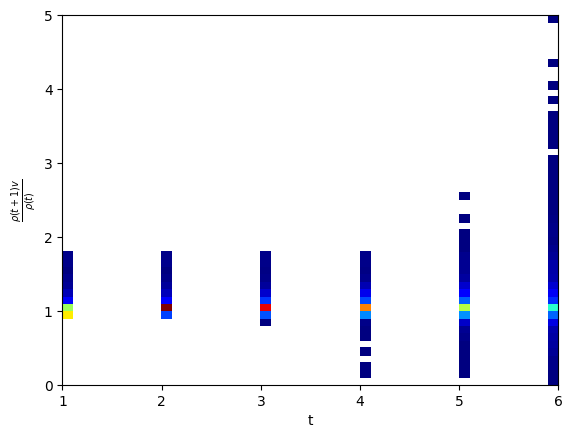
\includegraphics[width=\textwidth]{figures/AllDataNormalizedrunratio.png}
            \end{figure}
        \end{column}
        \begin{column}{0.45\textwidth}
        \begin{center}
            $g = v$ primes.
        \end{center}
            \begin{figure}
                \centering
                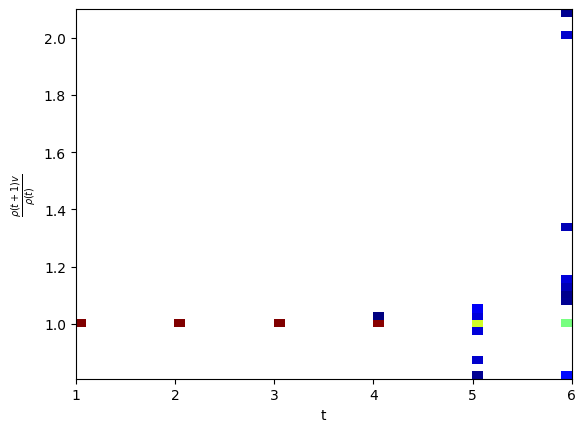
\includegraphics[width=\textwidth]{figures/AllDataAndvisGenNormalizedrunratio.png}
            \end{figure}
        \end{column}
    \end{columns}
    \begin{center}
                Distribution of $\rho(t+1)v/\rho(t)$ as a heatmap with $2 \leq v \leq 8$
    \end{center}
\end{frame}

\begin{frame}{ElGamal Sequences run ratio Experiment}
    \begin{columns}
        \begin{column}{0.45\textwidth}
        \begin{center}
            All primes.
        \end{center}
            \begin{figure}
                \centering
                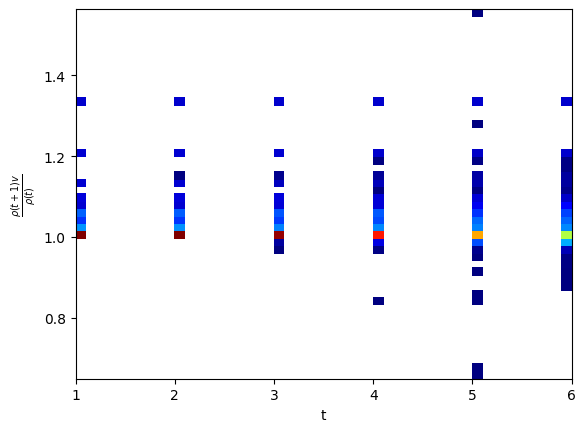
\includegraphics[width=\textwidth]{figures/v2Normalizedrunratio.png}
            \end{figure}
        \end{column}
        \begin{column}{0.45\textwidth}
        \begin{center}
            $g = v$ primes.
        \end{center}
            \begin{figure}
                \centering
                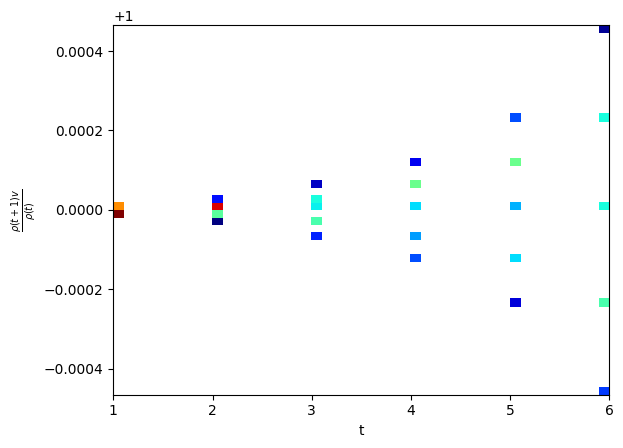
\includegraphics[width=\textwidth]{figures/v2AndvisGenNormalizedrunratio.png}
            \end{figure}
        \end{column}
    \end{columns}
    \begin{center}
                Distribution of $\rho(t+1)v/\rho(t)$ as a heatmap with $v = 2$
    \end{center}
\end{frame}
 	

%%% Local Variables:
%%% TeX-master: "../main.tex"
%%% End:
